\documentclass[oneside]{book}
\usepackage{../lal,fancyhdr,epsfig,psfig,color,hyperref,makeidx}
\includeonly{std,support,sample,hello,factories,tdfilters}

%define page size
\setlength{\textheight}{9.0in}
\setlength{\textwidth}{6.0in}
\setlength{\topmargin}{-0.00in}
\setlength{\oddsidemargin}{-0.25in}
\setlength{\evensidemargin}{\oddsidemargin}
\sloppy

\pagestyle{fancy}
\fancyhf{}
\lhead{\bf\nouppercase\rightmark}
\rhead{ \bf Pg \thepage}

\makeindex

\def\rcs#1{\def\next##1#1{\mbox{##1}}\next}
\newfont{\lsdfont}{cmbx10 at 72pt}

\begin{document}

% \reversemarginpar
% \let\marginpar\mparorig
% \providecommand{\marginpar}[1]{\mbox{}\mparorig{\raggedleft\hspace{0pt}#1}}

% The title page:
\title{
\vspace*{-1.0in}
\sffamily\bfseries\Huge
\textcolor{red}{\lsdfont L}AL
\raisebox{-2.5ex}{\textcolor{green}{\lsdfont S}\hspace{-0.1em}oftware}
\hspace{-2em}
\raisebox{-0.5ex}{\textcolor{blue}{\lsdfont D}\hspace{-0.2em}ocumentation} \\
\vspace*{-4.0in}
\center{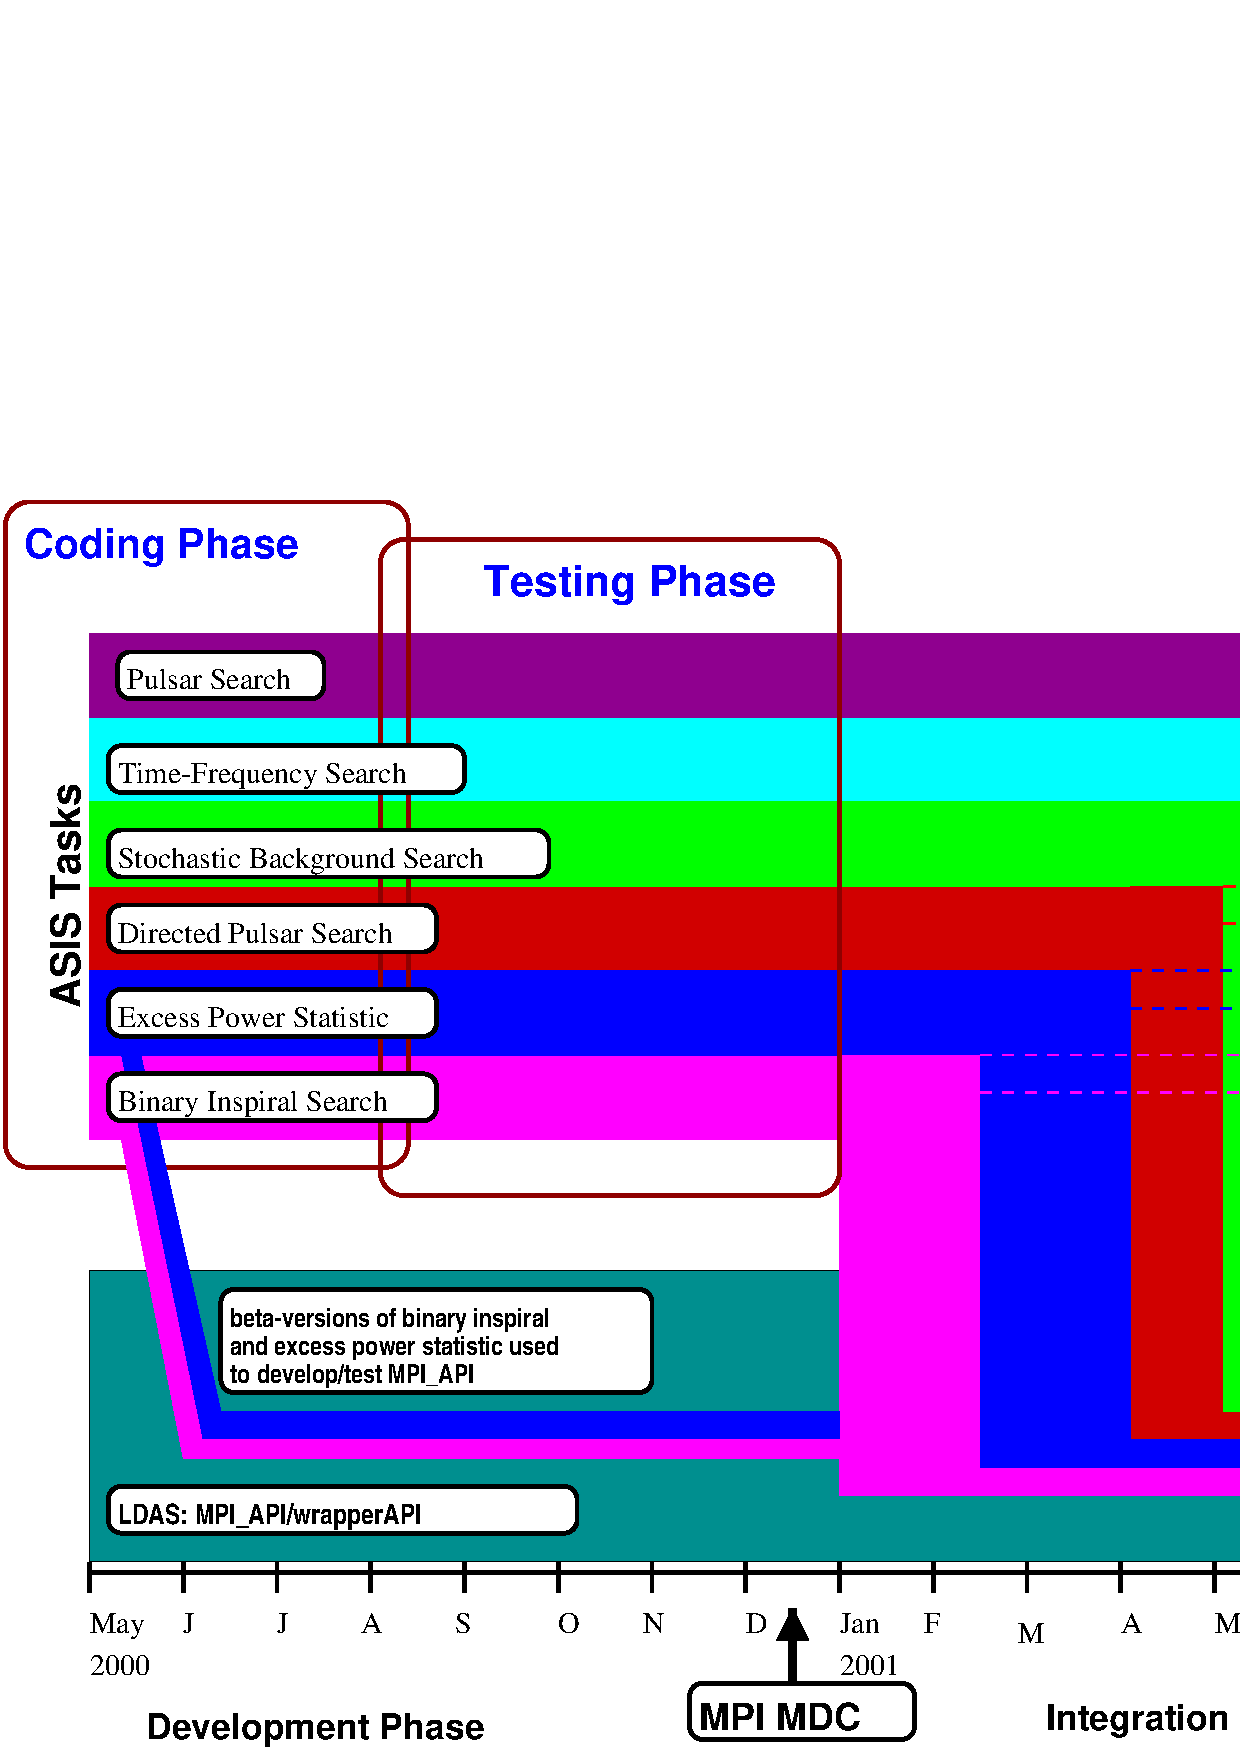
\includegraphics[width=1.2\linewidth,angle=0]{schedule} }
}
\author{\bf Members of the LSC}
\date{RCS \rcs$Revision$\rcs$Date$UTC --- Compiled:
\number\year/\ifnum\month<10 0\fi\number\month/\ifnum\day<10 0\fi\number\day}
\maketitle



% The table of contents.
\tableofcontents

\chapter*{Preface}
This is the LIGO/LSC Algorithm Library (LAL) Software Documentation.
The formal document governing LAL-code and documentation is the {\bf
LIGO Data Analysis System Numerical Algorithms Library Specification
and Style Guide}
\verb@http://www.ligo.caltech.edu/docs/T/T990030-07.pdf@ (called the
LAL-Spec through out).  Like a constitution describing a government,
the guidelines given in the LAL-Spec are quite general. What is given
here is a more like the criminal code: the nut-n-bolts explanation of
how to put the LAL-Spec into practice.  Like a constitution, {\bf if
there are any inconsistencies,  the LAL-Spec takes precedence over any
statements in this document.} Also like the constitution, if there is
something that really needs to be changed in the LAL-Spec, it can be
changed.

The first part of this document gives a brief introduction to the LAL
and some coding and documentation instructions.  The second part is
the documentation of the LAL code itself.

\part{Coding and Documentation Instructions}

\chapter{Finding your way through the LAL}

\section{The LAL webpage}

An up to date release  of the LAL -- and a wealth of other information
-- can be obtained from the LAL webpage
\verb@http://www.lsc-group.phys.uwm.edu/lal/@

\begin{itemize}
   \vspace*{-0.1in}
    \item[$\bullet$ ]  {\bf Current distribution"} You can can click
                       to down load the tar ball.
    \vspace*{-0.051in}
    \item[$\bullet$ ] {\bf LAL software librarian:}  You can click to
                      email the librarian.
    \vspace*{-0.051in}
    \item[$\bullet$ ] {\bf The CVS tree:}  You can use this to insure 
                      that you are working on the latest version
                      any file in within the LAL.
    \vspace*{-0.051in}
    \item[$\bullet$]  {\bf Previous releases of LAL:} If you want an older 
                      version for sentimental reasons, you can find it here.
    \vspace*{-0.051in}
    \item[$\bullet$ ] {\bf Data:}  You can surf to the LIGO data archive to get
                      data.  There is a short snippet of 40-m data called 
                      {\tt lal.small} for testing.  This snippet of data 
                      is not subject to the access restrictions that some 
                      of the others are.
    \vspace*{-0.051in}
    \item[$\bullet$ ] {\bf Links to other useful software:} In order to
                      fully use the LAL, you will need to install the
                      these packages:
    \begin{itemize} 
          \vspace*{-0.051in}
          \item {\texttt {FFTW}}:  Fastest Fourier Transform in the West
          \vspace*{-0.051in}
          \item {\texttt {MPI}}:  The parallel code implementation
          \vspace*{-0.051in}
          \item {\texttt {frames}}: Package for reading frame format data
    \end{itemize} 
\end{itemize}

\section{Version control}

As required by the LAL-Spec, the LAL is kept in a CVS repository;
however, at present, the software Librarian has the only key.
Individual users can only ``check in'' code by sending it to him.
Although we will likely change this policy in the future, we have
sound reasons for doing it this way now. 

It is important that the code in the repository reflect the software
standard as closely as possible.  Since the standard is new, changing,
and sometimes unclear, we feel it is a good policy to have the
Librarian look over the code submissions before they become publically
available and possibly immitated.

Another reason for limiting user access to the CVS is portability of
the code.  Thus far, the LAL librarian has been fastidious in making
sure that all the code in  LAL compiles and runs on almost anything.
For now, we would like to keep it that way, and this is easier to do
incrementally from the start, rather than trying to fix a big mess
later.

Although users do have to go through the librarian to check code in,
they have easy access to the latest ``Librarian-approved'' code on the
from the CVS tree on the web page. (See above.)

\section{Installing LAL on your machine}

When you down load the LAL package, you will find the installation
instructions in the file {\tt /lal/INSTALL}.

\chapter{Notes about coding}
\label{c:CodingNotes}

As mentioned above,  the marching orders for code development laid out
in the LAL-Spec are too general and often vague.  The purpose of this
chapter is try to record the collective interpretation of the LAL-Spec
so  that we can consistantly apply it.

\bigskip

{\noindent \bf Use of MACROS:} The LAL-Spec says ``macros'' are
deprecated.  What the hell does that mean? The interpretation we are
using clearly captures the intent.  There are a number of macros for
common use in the {\tt std} LAL files, but these under strict control
of the librarian.  In your modules (.c files), you may use macros to
replace small snippets of code.  However because header files may be
included in other code, you should not use macros in your {\tt .h}
files.

If you have a ``{\texttt {\#define SomeMacro}}'' that needs to be
included in many different files, it probably belongs in the {\tt
LALConstant.h} file or one of the other {\tt /lal/std/include} files.
Please contact the Librarian.

\bigskip

{\noindent \bf Defining the RCS ID string:}  The LAL-Spec says this
must be done in all header, module and test files. To do this you must
use:
\begin{verbatim}
          NRCSID(LALTEMPLATEH,"$Id$");
\end{verbatim}
\noindent The reason we assign the Id with this macro is that without it,
the compiler prints annoying warning messages. Note this macro is an
example of one macros for ``common use'' described above.

\bigskip

{\noindent \bf Error Codes and Messages:} The LAL-Spec discusses
statuscode and statusDesription. Here we solidify the name space
convention. These should be hash-defined in the header file,
eg in {\tt MyHeader.h} we would have
\begin{verbatim}
/* <lalErrTable file="MyHeaderHErrorTable"> */

#define MYHEADERH_ENUL  1 
#define MYHEADERH_EOUT  2
#define MYHEADERH_EDIV  3

#define MYHEADERH_MSGENUL  "Null pointer"
#define MYHEADERH_MSGEOUT  "Output already exists"
#define MYHEADERH_MSGEDIV  "Division by zero"

/* </lalErrTable> */
\end{verbatim}
\noindent The names should begin with the file name and extention ({\tt h})
all converted to upper case. The error codes are followed by
{\tt \_E}$<$name$>$. The error messages are followed by
{\tt \_MSGE}$<$name$>$.

The key-words shown before and after the codes are the key-words for
extracting this information for automatically including it in the
documentation. You must automate the inclusion of these in the
documentation.

\chapter{The directory structure of the LAL}
\label{c:DirectoryStructure}

\newpage
\section{Schematic Diagram of Directory Structure}
This is the  directory structure is laid out in the LAL Spec.
\noindent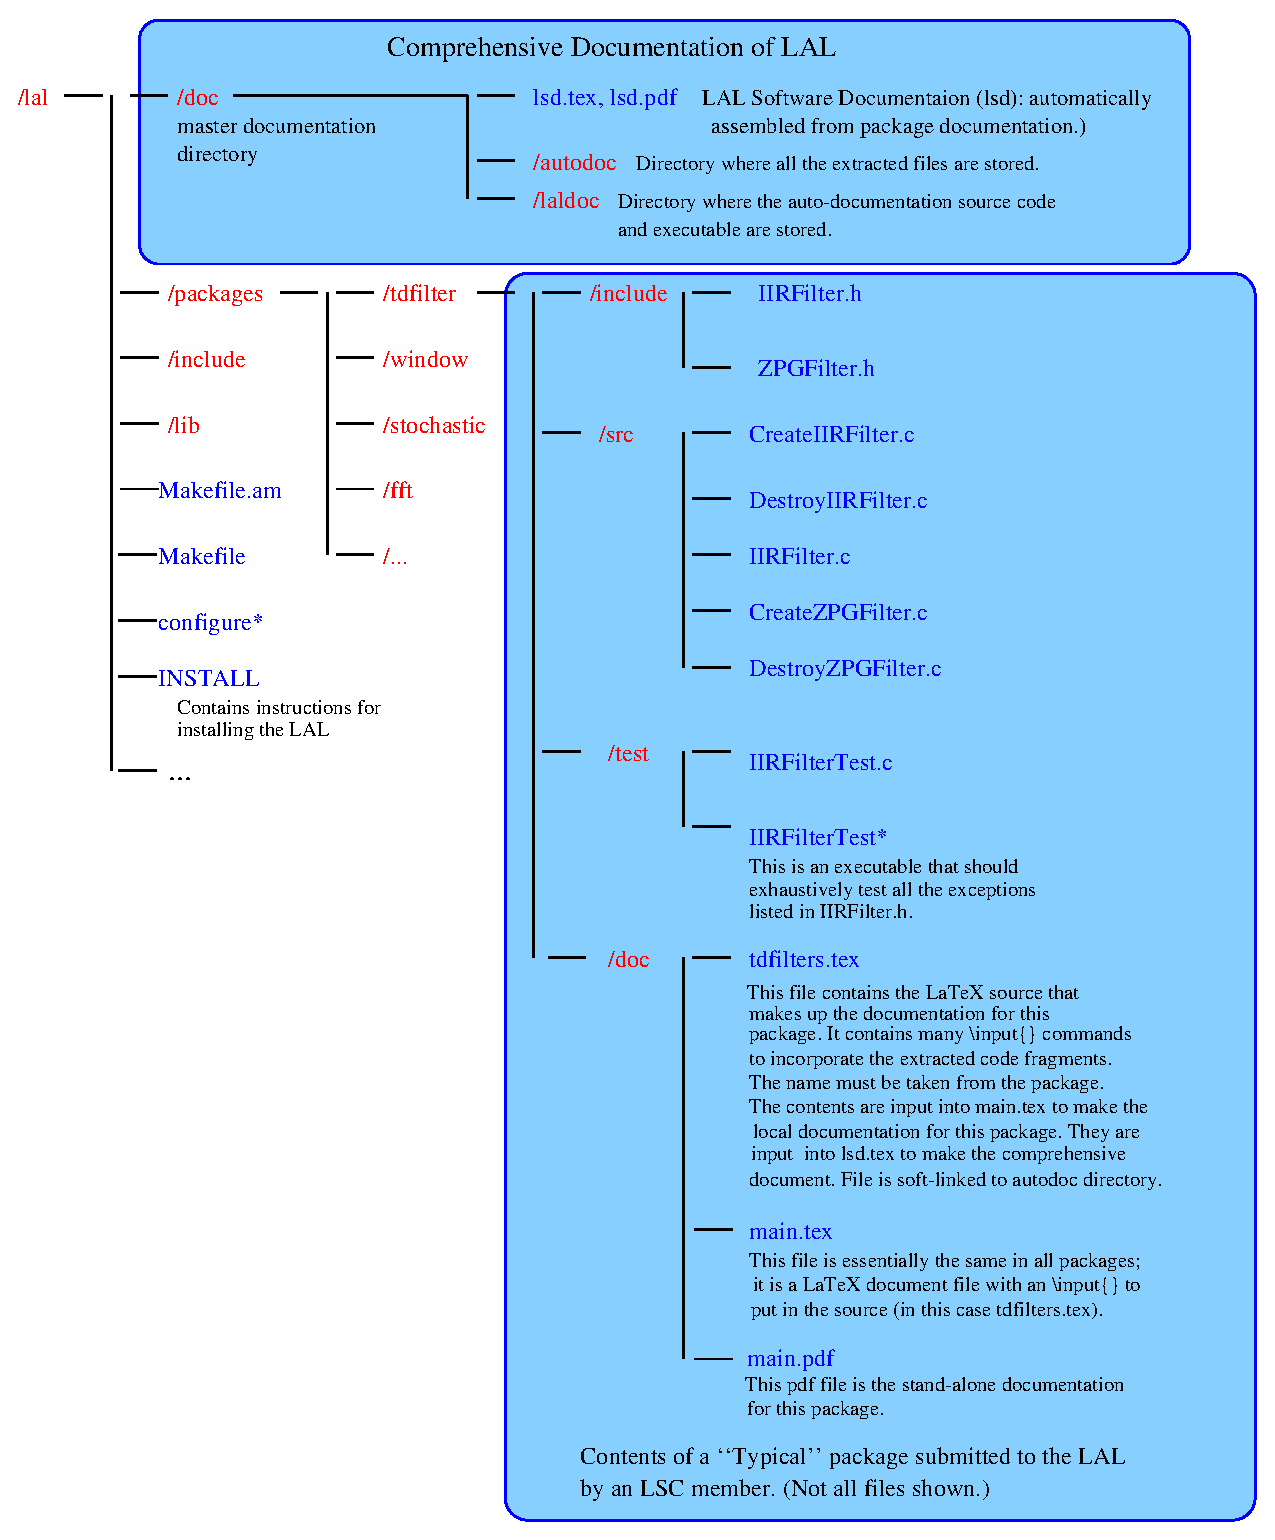
\includegraphics[width=0.9\linewidth,angle=0]{lsdFigDirStructure}

\chapter{Documenting your code}
\label{c:DocumentingCode}

Along with any code submission to the LAL library, you will need to
supply documentation. Keep in mind, the documentation, like the code,
is a {\it deliverable} and it must be written to the standard outlined
in the LAL-Spec.  This chapter gives specific instructions  on how 
to meet standard.

Also keep in mind that, unlike most code projects that physicists work
on, this code may still need to be maintained long after the author
has been denied tenure and starts working for a dot-com company.  This
puts a heavy burden on the documentation: not only should it help you
maintain your code, but it should require minimum effort for {\it
anyone} to figure out how the code works and how to fix it. If you
find yourself saying ``The easiest way for me to maintain my code is
...'', you have missed the point.


In this chapter we discuss a few prelinaries, and give a general
outline of the documentation for a package.  Chapter
\ref{c:SamplePackage} is an example of how a the documentation for a
LAL package should be laid out. In Chapter \ref{c:laldoc} we explain
how to use the auto-documentation system ({\tt laldoc}).

\section{Use \LaTeX}

The documentation should be written in \LaTeX. This decission was made
by the LSC software committee.  The primary reason for this choice was
the need for the equation-writing capablility of \LaTeX.

The danger in using \LaTeX  is that not everyone will have the same
version of \LaTeX installed on their machine. [Actually, this problem
might be as bad, or worse, with some other documenting tool.] To try
to minimize this problem, stick with the vanilla \LaTeX as best you
can.

Within the LAL distribution we supply a class file ({\tt
lal/doc/lal.sty}).  Although this is helpful and it makes thing look
nicer, it is not essential. You can remove it from the
\verb@\usepackage[]@ command and the \LaTeX should work without it.

\newpage
\section{The lay out of the documentation}

The hierarchical lay out of the documentation exactly follows the
hierarchy of the code.

\begin{itemize}
    \vspace*{-0.1in}
    \item Documentation for the N'th package forms chapter {\large \bf N}. 
    \vspace*{-0.051in}
    \begin{itemize} 
        \vspace*{-0.051in}
        \item Documentatin of header1.h in the package forms section
             {\large \bf N.1}.
             \begin{itemize} 
                 \vspace*{-0.051in}
                 \item Documentation of Module1.1 that 
                       ``{\texttt {\#include}}'s'' header1.h
                       is in subsection {\large \bf N.1.1}.
                 \vspace*{-0.051in}
                 \item Documentation of Module1.2 that 
                       ``{\texttt {\#include}}'s'' header1.h
                       is in subsection {\large \bf N.1.2}.
                 \vspace*{-0.051in}
                 \item ... additional modules.
             \end{itemize} 
        \vspace*{-0.051in}
        \item Documentatin of header2.h in the package forms section.
             {\large \bf N.2}.
             \begin{itemize} 
                 \vspace*{-0.051in}
                 \item Documentation of Module2.1 that 
                       ``{\texttt {\#include}}'s'' header1.h
                       is in subsection {\large \bf N.2.1}.
                 \vspace*{-0.051in}
                 \item Documentation of Module2.2 that 
                       ``{\texttt {\#include}}'s'' header1.h
                       is in subsection {\large \bf N.2.2}.
                 \vspace*{-0.051in}
                 \item ... additional modules
             \end{itemize} 
        \vspace*{-0.051in}
        \item Documentatin of header3.h in the package forms section.
             {\large \bf N.3}.
             \begin{itemize} 
                 \vspace*{-0.051in}
                 \item ... additional modules
             \end{itemize} 
        \vspace*{-0.051in}
        \item ... additional headers
    \end{itemize} 
    \vspace*{-0.1in}
    \item Documentation for the N+1'th package forms chapter {\large \bf N+1}. 
    \item ... additional packages
\end{itemize}


\section{What about figures?}

Figures are fine. When you submit a package of code and documentation
the figures should be in the {\tt /lal/packages/mypackage/doc} directory.
Please submit two versions of the figure: an {\tt .eps} and a {\tt .pdf}.
We need both so we can build the documentation either with 
\LaTeX or {\tt pdflatex}.

The syntax to use for putting in the figure should be something like this
\begin{verbatim}
\noindent\includegraphics[width=0.9\linewidth,angle=0]{MyHeaderFileNameMyFig}
\end{verbatim}
Note. Don't include the extension on the figure file name in
the \verb@\includegraphics[]{}@ command. If you leave the extension off, 
whatever method you use for building the documentation automatically
looks for the appropriate file.

{\bf Naming convention for figure files:} Using the base name of the
header file as the first part of the figure file name is a good idea.
The reason: when the documentation is built, everything is {\LaTeX}ed
in  the {\tt lal/doc/autodoc} directory. There are hundreds of files there,
and  following this convention will reduce the probability of a
name-space collision.

\section{Autodocumentation and Indexing }

\subsection{Autodocumentation requirements}
There is an automatic documentation tool supplied with the LAL.
To what extent the coders wish to use the autodocmentation system,
is largely left up to their judgement and patience. However, there
are a few things that must be autodocumented.

\begin{itemize}
  \item[$\bullet$] {\bf Function Protoypes} 
  \item[$\bullet$] {\bf Error code tables }
  \item[$\bullet$] {\bf The author and version-control information.}  This
                        should appear as footnote at the bottom of all
                        header sections, and module and test subsections.
                        This can be done with the \LaTeX command 
                        \verb@\vfill{\footnotesize\input{MyFileHAuthVer}}@,
                        where {\tt MYFILEHAuthVer.tex} is the file where
                        the Author-Version information from {\tt MyFile.H}
                        was extracted to.
\end{itemize}

\subsection{Indexing requirements}

When this  document is built an index is also constructed. There are a few
code items that you must place in the index.
\begin{itemize}
  \item[$\bullet$] {\bf Functions} must be entered in the index, so
   users can find them. The \verb@\index{}@ command should be right
   after the prototypes themselves are entered.  This insures the page
   number that appear in the index will be the page where the
   prototype is explained in the document.
   Use the \LaTeX command
  \begin{verbatim}
  \index{{\texttt MyFunction()} You can put a short explantory string here.}
  \end{verbatim}
  \vspace*{-0.041in}
  \item[$\bullet$] {\bf Non LAL Data Structures}  must appear in the index.
  The \verb@\index{}@ command should be right after in the section
  where they are explained in the documentation.
  Use the \LaTeX command
  \begin{verbatim}
  \index{{\textt MyStruct} You can put a short explantory string here.}
  \end{verbatim}
\end{itemize}






\chapter{Package {\texttt {samplepackage}}}
\label{c:SamplePackage}

An introductory description of what is in the package.
There is no specific length limit, but $O[1]$ page seems
reasonable. Note the naming conventions for packages: all lower case. 


\newpage

\section{Header {\texttt {SampleHeader1.h}}}
Put a one sentence description of the header right after the section
heading.

\subsection*{Synopsis}

\begin{verbatim}
#include "SampleHeader1.h"
\end{verbatim}
Since it is possible that a few modules will use the same header file
you can put a general discription of what is to come here.

\subsection*{Error conditions}
To insure that these are current with the code, a table of {\bf these
must be automatically extracted from the source code with the {\tt
laldoc} autodocumentor.}

Additional explanation (if necessary) of the error conditions can
follow the table.

\subsection*{Structures}

If there are any non LAL structures declared in the header, they must
be documented here.  They must also be included in the index with a
\verb@\index{sampleStruct}@ \LaTeX command.

\vfill{\footnotesize{
\vspace{-1ex}
\mbox{}\marginpar{\tiny\texttt{l.1}\\\texttt{SampleHeader1.h}}
\vspace{-3ex}
\begin{verbatim}
Author: Hacker, A. Good
$Id$
\end{verbatim}
}}

\newpage

\subsection{Module {\texttt {SampleModule1.c}}}
Put a one sentence discription explaining what this module will do. 
[Also, start a new page for documenting each module.]

\subsection*{Prototypes}
{\bf Function prototypes must be extrated verbatim from
the source code and "{\verb@\input{}@}" here.}

{\bf Every function must be placed into the index with
a \verb@\index{SampleFunction()}@ \LaTeX command.}

\subsection*{Description and operating instructions}
Describe the arguments of the function, and how to use the function.
Remember to document any non LAL {\tt structs} in the header
file documentation.

\subsection*{Algorithm}
Explanation of the algorithm.

\subsection*{Uses}
A list of all the other routines that this module uses.

\subsection*{Notes}

\subsection*{Validation Information}

This section will be formally filled in when the code is officially
validated. In the mean time, if you have timing or bench-mark testing
information, put it here.


\vfill{\footnotesize{
\vspace{-1ex}
\mbox{}\marginpar{\tiny\texttt{l.1}\\\texttt{SampleModule1.c}}
\vspace{-3ex}
\begin{verbatim}
Author: Hacker, A. Good
$Id$
\end{verbatim}



\newpage

\subsection*{Program {\texttt {SampleTest.c}}}
Breif description, e.g. "Performs tests on all routines in SampleHeader.h."

\subsection*{Usage}
Show and explain the command line syntax used to run the program.

\subsection*{Description and operating instructions}
Explanation of the algorithm.



\subsection*{Exit Codes}

A table containing all the exit codes for the program.  We strongly
suggest that the exit codes be coded in exactly the same way as the
error codes in the header file.  If you do this you can use the {\tt
laldoc} Error Table tool to build a table to insert here. (See below.)
If you don't use {\tt laldoc} to make the table, please LaTeX it by
hand.

The table may followed with additional explanation.

\subsection*{Uses}

A list of all the other routines that this module uses.

\subsection*{Notes}


\vfill{\footnotesize{
\vspace{-1ex}
\mbox{}\marginpar{\tiny\texttt{l.1}\\\texttt{SampleTest.c}}
\vspace{-3ex}
\begin{verbatim}
Author: Hacker, A. Good
$Id$
\end{verbatim}


\chapter*{References}

A bibliography all the references used in the Package {\tt samplepackage}.

\chapter*{Index}
The index for the Package {\tt samplepackage} comes here.

The \verb@\printindex@ command should be in the {\tt main.tex} file.
This should start on a new page.


\chapter{The automatic documentation system {\texttt {laldoc}}, and how to use it.}
\label{c:laldoc}

\section{A four step introduction to {\texttt {laldoc}} }

\begin{itemize}
\item[(1)] Copy the executable ({\tt /lal/doc/laldoc/laldoc}) 
and the  sample input file ({\tt /lal/doc/laldoc/LalDocDemo.h}) to an
empty  {\tt /junk} directory.
\item[(2)] In {\tt /junk} run the command ``\verb@./laldoc Input.h Errors.out@'' 
\item[(3)] \LaTeX the file {\texttt {LalDocDemo\_LaTeX\_This\_File.tex}}
and look at it.
\item[(4)] Examine the input file and the various debris files created.
You will see exactly what  {\texttt {laldoc}} does.
\end{itemize}

\section{Brief Discription of {\texttt {laldoc}} }

The auto-documentor is designed to let LAL programmers extract
fragments of code or comments from the source files and include them
in their documentation.  This is done in such a way that if the
fragment in the source code is modified, then the change is
automatically incorporated into the documentation the next time the
document is built.  

This extraction is  accomplished by having the programmer surround the
fragments of code he or she wishes to incorporate in the document with
key-words.  Currently, we only have three pairs of key-words, so the
learning curve is flat and short! The source code (the .c and .h
files) is then parsed and the fragments written to storage files.
(The key-word also includes a user-specified file name for this
storage file.)  When you write your \LaTeX document simply use the
\LaTeX command \verb@\input{}@ to put the contents of the storage file
in the document where you need it.  [If you have installed the LAL
software package, you can see all the extracted storage files in the
directory {\tt lal/doc/autodoc}.]

\subsection{ The {\texttt {laldoc}} command line }
The full functionality of the command line is:
\begin{verbatim}
     laldoc inputFile.c errorFile /home/alice/errorDir/ /home/alice/inputDir/
\end{verbatim}
\noindent
The first argument is the input file name, the second is an error reporting
file, the third argument is the directory where the errorfile will be
written, and the fourth is the directory where {\tt laldoc} will look
for the input file.  The third and the fourth arguments are optional.


\subsection{ The three {\texttt {laldoc}} environments }
\begin{description}
\item[$\bullet$ ]
{\tt <lalVerbatim file="myVerbatimJunk">}  and {\tt </lalVerbatim> }
This wraps the  material between the two key-words in a \LaTeX {\tt
verbatim} environment for later inclusion.  This is useful for
including such things as a function protypes or data structures: the
documentation will include them ``verbatim''.  When the information is
included with {\tt <lalVerbatim>} a small {\tt marginpar} gives the
source-file name and line number where the snippet came from.
\vspace*{-0.05in}
\item[$\bullet$ ] 
{\tt  <lalLaTeX file="myLatexJunk">}   and {\tt </lalLaTeX > } This is
used to write \LaTeX in the source-code. The material between the two
key-words is stored in a file {\tt myLatexJunk.tex}.  This allows (not
recommended) a programmer to put large sections of \LaTeX pros in the
source code.  
\vspace*{-0.05in}
\item[$\bullet$ ] 
{\tt <lalErrTable file="myErrTabJunk">} and {\tt </lalErrTable> } This
does extensive parsing of the code to assemble a \LaTeX table from the
source code where the error conditions are defined.  This insures that
if an error code is added in the source, it will automatically be
added to the documentation.
\vspace*{-0.051in}
\end{description}

\subsection{ How {\texttt {laldoc}} handles the output files}

{\bf Default file names:} In any of the {\texttt {laldoc}} enviroments,
if you do not specify an output file in the opening key-word line,
{\texttt {laldoc}} will assign one automatically. The file name will
be constructed from the input file name, e.g. if the input
is  {\tt MyHeader.h}, the output will be  {\tt MyHeaderH.tex}.

{\bf Appending to files:}
If the output file doesn't already exist, {\texttt {laldoc}} will
create it.  If the output file already exists, {\texttt {laldoc}} will
append to it.  When the environment-closing key-word is encountered,
the output file is closed.

Although this is a fairly obvious feature, it is quite useful.  For
example, the function prototypes in a module don't appear to together,
but they should appear together in the documentation.  With {\texttt
{laldoc}} this is easy to accomplish. In your source code when you
encounter each prototype that must be captured for inclusion, use the
same file name for the extraction. Each protype will be appended after
the other, and seperate margin pars will tell exactly where each came
from, i.e surround each prototype with the pair
{\tt <lalVerbatim file="MyModuleCPrototypes">} {\tt </lalVerbatim>}.





\section{Examples of how to use the three environments in {\texttt {laldoc}} }

As with most things computer, the best way to learn how use the auto
documentor is to snoop around the source tree and find some examples,
and then try a few things.  The source code and the executable for the
parser ({\tt laldoc}), are in the directory {\tt lal/doc/laldoc}.  The
directory also has a README file that give some nuts-n-bolts
instructions on how to use the parser.  This sections gives the basics
of what you can do.


\subsection{The {\texttt {<lalVerbatim>} }  evironment }

As an example, look at the code fragment in the source file 
\texttt{lal/packages/tdfilter/src/CreateZPGFilter.c}.

\begin{verbatim}
/* <lalVerbatim file="CreateZPGFilterCP"> */
void CreateCOMPLEX8ZPGFilter(Status            *stat,
			     COMPLEX8ZPGFilter **output,
			     INT4              numZeros,
			     INT4              numPoles)
/* </lalVerbatim> */
\end{verbatim}
When {\tt laldoc} parses the source file, it produces the following
output in the file {\tt CreateZPGFilterCP.tex}

\begin{verbatim}

\vspace{-1ex}
\mbox{}\marginpar{\tiny\texttt{l.51}\\\texttt{CreateZPGFilter.c}}
\vspace{-3ex}
(backslash)begin{verbatim}
void CreateCOMPLEX8ZPGFilter(Status            *stat,
                             COMPLEX8ZPGFilter **output,
                             INT4              numZeros,
                             INT4              numPoles)
(backslash)end{verbatim}
\end{verbatim}

This is then included in the \LaTeX documentation with an
\verb@\input{CreateZPGFilterCP}@ command.

\vspace{-1ex}
\mbox{}\marginpar{\tiny\texttt{l.51}\\\texttt{CreateZPGFilter.c}}
\vspace{-3ex}
\begin{verbatim}
void CreateCOMPLEX8ZPGFilter(Status            *stat,
                             COMPLEX8ZPGFilter **output,
                             INT4              numZeros,
                             INT4              numPoles)
\end{verbatim}

The {\tt marginpar} on the far right tells the line number and file
name from which this fragment was extracted.

{\bf Note the naming convention used for the file where the extracted
code was stored: the base name comes from the file where it was
extracted (here {\texttt {CreateZPGFilter}}), followed by a ``C'' (in
this case to denote that it came from the .c file).  {\Large {Use This
Naming Convention!}} This will avoid most name-space collisions.}  In
this case,  the the ``P'' is for function {\it prototype}.


\subsection{The {\texttt {<lalLaTeX>} } evironment }

The {\texttt {<lalLaTeX>} } environment works much the same
was as the {\texttt {<lalVerbatim>} } environment. The the distinction
being that the extracted material should be valid \LaTeX ready
for insertion into a \LaTeX file. Unlike the 
{\texttt {<lalVerbatim>} } environment, no wrapping is supplied
by the parser.

Leading ``*'''s on a line will be stripped out by {\tt laldoc} in the
{\texttt {<lalLaTeX>}} environment. This is to accomodate the common
practice in c of putting leading ``*'''s on comment lines.  The way
this is done is {\tt laldoc} checks to see if the first non blank
character on the line is a ``*''. If it is, then it is replaced by
blank when the \LaTeX is written to the output file. The leading
blanks are then ignored by \LaTeX.


\subsection{The {\texttt {<lalErrTable>} } environment, for printing
a table of the error codes and warnings.}

See the example in Chapter \ref{c:CodingNotes}.





\part{Documentation of the LAL packages}
\chapter{Package \texttt{std}}

This package contains headers providing basic datatypes, constants,
and macros that support the LAL standard.

\newpage\input{LALStdlibH}
\newpage\input{LALRCSIDH}
\newpage\input{LALDatatypesH}
\newpage\input{LALStatusMacrosH}
\newpage\input{LALConstantsH}
\newpage\input{LALStdioH}
\newpage\input{LALVersionH}
\newpage\input{LALMallocH}
\newpage\input{LALErrorH}
\newpage\input{LALGSLH}
\newpage\input{StringInputH}


\newpage\begin{thebibliography}{0}
\bibitem{Barnet:1996}
  Particle Data Group, R.~M. Barnett et al., Phys. Rev. D\textbf{54},
  1 (1996)
\bibitem{Lang:1992}
  K.~R. Lang, \textit{Astrophysical Data: Planets and Stars}.
  Springer-Verlag, New York (1992)
\end{thebibliography}

\chapter{Package \texttt{support}}

%% $Id$

This package covers LAL support routines.

These routines do not conform to LAL requirements, and many of them should be
used only for debugging and in test code, not in production code.  These are
compiled and installed as a separate library \texttt{lalsupport}.

\newpage\input{LALStdioH}
\newpage\input{LALVersionH}
\newpage\input{LALMallocH}
\newpage\input{LALErrorH}
\newpage\input{GridH}
\newpage\input{PrintVectorH}
\newpage\input{PrintFTSeriesH}
\newpage\input{ReadFTSeriesH}
\newpage\input{ReadNoiseSpectrumH}
\newpage\input{StringInputH}
\newpage\input{StreamInputH}
\newpage\input{StreamOutputH}
\newpage\input{LALInitBarycenterH}
\newpage\input{LALXMGRInterfaceH}
\newpage\input{LIGOLwXMLH}
\newpage\input{LIGOLwXMLReadH}
\newpage\input{SFTfileIOH}
\newpage\input{ConfigFileH}
\newpage\input{UserInputH}
\newpage\input{LALMathematicaH}

\chapter{Package \texttt{sample}}

This package contains templates for LAL headers and modules, as well
as a fully-autodocumenting example program based on the primer in the
\verb@std@ package.

\newpage\input{LALSampleH}

\section{Program \texttt{lalapps\_hello}}
\label{program:lalapps-hello}
\idx[Program]{lalapps\_hello}

\begin{entry}

\item[Name]
\verb$lal_hello$ --- prints ``hello LSC!''

\item[Synopsis]
\verb$lal_hello$ [\verb$-h$] [\verb$-V$] [\verb$-v$]
[\verb$-d$ \textit{dbglvl}] [\verb$-o$ \textit{outfile}]

\item[Description]
\verb$lal_hello$ prints ``hello LSC!'' to the screen or to an output file.

\item[Options]\leavevmode
\begin{entry}
\item[\texttt{-h}]
Print a help message.
\item[\texttt{-V}]
Print the version information.
\item[\texttt{-v}]
Verbose output.
\item[\texttt{-d} \textit{dbglvl}]
Set LAL debug level to \textit{dbglvl}.
\item[\texttt{-o} \textit{outfile}]
Write the output to file \textit{outfile}.
\end{entry}

\item[Debug levels]
The LAL debug level can be specified as an integer or as a string of flags:
\begin{entry}
\item[\texttt{NDEBUG}]
No debugging information is printed and memory debugging code is disabled.
\item[\texttt{ERROR}]
Error messages are printed.
\item[\texttt{WARNING}]
Warning messages are printed.
\item[\texttt{INFO}]
Information messages are printed.
\item[\texttt{TRACE}]
Function call tracing messages are printed.
\item[\texttt{MEMINFO}]
Memory  allocation  information messages are printed.
\item[\texttt{MEMDBG}]
Debugging of memory allocation routines is enabled but no messages are printed.
\end{entry}
The following composite levels are available:
\begin{entry}
\item[\texttt{MSGLVL1}]
Equivalent to \verb$ERROR$
\item[\texttt{MSGLVL2}]
Equivalent to \verb$ERROR | WARNING$
\item[\texttt{MSGLVL3}]
Equivalent to \verb$ERROR | WARNING | INFO$
\item[\texttt{ALLDBG}]
All debugging messages are printed.
\end{entry}

For example, the command
\begin{indented}
\verb$lal_hello -d "ERROR | INFO"$
\end{indented}
will set the debug level so that error and information messages are printed.

\item[Environment]\leavevmode

\begin{entry}
\item[\texttt{LAL\_DEBUG\_LEVEL}]
Default LAL debug level to use.
\end{entry}

\item[Author]
Jolien Creighton

\end{entry}

\chapter{Package \texttt{factories}}

This package provides routines for creating and destroying the LAL aggregate
datatypes.

\newpage\input{AVFactoriesH}
\newpage\input{SeqFactoriesH}

%\chapter{Package \texttt{vectorops}}

This package contains routines for manipulating vectors.

\newpage\input{VectorOpsH}
\newpage\input{VectorIndexRangeH}
\newpage\begin{thebibliography}{0}
\bibitem{ptvf:1992}
  W. H. Press, S. A. Teukolsky, W. T. Vetterling, and B. P. Flannery,
  \textit{Numerical Recipes in C: The Art of Scientific Computing}, 2nd ed.
  (Cambridge University Press, Cambridge, England, 1992).
\end{thebibliography}

%\chapter{Package \texttt{utilities}}

This package contains various numerical utilities for use in LAL.

\newpage\input{RandomH}
\newpage\input{FindRootH}
\newpage\input{IntegrateH}
\newpage\input{InterpolateH}
\newpage
\section{Header \texttt{Sort.h}}

Provides routines for sorting, indexing, and ranking real vector
elements.

\subsection{Synopsis}
\begin{verbatim}
#include "Sort.h"
\end{verbatim}


\subsection{Error conditions}
\begin{tabular}{|c|l|l|}
\hline
status & status                      & Explanation                      \\
 code  & description                 &                                  \\
\hline
\tt 1  & \tt Null pointer            & Missing a required pointer.      \\
\tt 2  & \tt Length mismatch         & Vectors are of different length. \\
\tt 3  & \tt Memory allocation error & Could not allocate memory.       \\
\hline
\end{tabular}

\subsection{Structures}
\newpage
\subsection{Module \texttt{HeapSort.c}}

Sorts, indexes, or ranks vector elements using the heap sort
algorithm.

\subsubsection{Prototypes}
\vspace{0.1in}
\input{HeapSortD}

\subsubsection{Description}

These routines sort a vector \verb@*data@ (of type \verb@REAL4Vector@
or \verb@REAL8Vector@) into ascending order using the in-place
heapsort algorithm, or construct an index vector \verb@*index@ that
indexes \verb@*data@ in increasing order (leaving \verb@*data@
unchanged), or construct a rank vector \verb@*rank@ that gives the
rank order of the corresponding \verb@*data@ element.

The relationship between sorting, indexing, and ranking can be a bit
confusing.  One way of looking at it is that the original array is
ordered by index, while the sorted array is ordered by rank.  The
index array gives the index as a function of rank; i.e.\ if you're
looking for a given rank (say the 0th, or smallest element), the index
array tells you where to look it up in the unsorted array:
\begin{verbatim}
unsorted_array[index[i]] = sorted_array[i]
\end{verbatim}
The rank array gives the rank as a function of index; i.e.\ it tells
you where a given element in the unsorted array will appear in the
sorted array:
\begin{verbatim}
unsorted_array[j] = sorted_array[rank[j]]
\end{verbatim}
Clearly these imply the following relationships, which can be used to
construct the index array from the rank array or vice-versa:
\begin{verbatim}
index[rank[j]] = j
rank[index[i]] = i
\end{verbatim}

\subsubsection{Algorithm}

These routines use the standard heap sort algorithm described in
Sec.~8.3 of Ref.~\cite{ptvf:1992}.

The \verb@SHeapSort()@ and \verb@DHeapSort()@ routines are entirely
in-place, with no auxiliary storage vector.  The \verb@SHeapIndex()@
and \verb@DHeapIndex()@ routines are also technically in-place, but
they require two input vectors (the data vector and the index vector),
and leave the data vector unchanged.  The \verb@SHeapRank()@ and
\verb@DHeapRank()@ routines require two input vectors (the data and
rank vectors), and also allocate a temporary index vector internally;
these routines are therefore the most memory-intensive.  All of these
algorithms are $N\log_2(N)$ algorithms, regardless of the ordering of
the initial dataset.


\subsubsection{Uses}
\begin{verbatim}
I4CreateVector()
I4DestroyVector()
\end{verbatim}

\subsubsection{Notes}


\newpage
\subsection{Program \texttt{SortTest.c}}

A program to test sorting routines.

\subsubsection{Usage}
\begin{verbatim}
SortTest [-s seed] [-d [debug-level]]
\end{verbatim}

\subsubsection{Description}

This test program creates rank and index arrays for an unordered list
of numbers, and then sorts the list.  The data for the list are
generated randomly, and the output is to \verb@stdout@ unless
redirected.  \verb@SortTest@ returns 0 if it executes successfully,
and 1 if any of the subroutines fail.

The \verb@-s@ option sets the seed for the random number generator; if
\verb@seed@ is set to zero (or if no \verb@-s@ option is given) then
the seed is taken from the processor clock.  The \verb@-d@ option
increases the default debug level from 0 to 1, or sets it to the
specified value \verb@debug-level@.


\subsubsection{Algorithm}

\subsubsection{Uses}
\begin{verbatim}
debuglevel
CreateI4Vector()
CreateSVector()
DestroyI4Vector()
DestroySVector()
CreateRandomParams()
DestroyRandomParams()
UniformDeviate()
LALPrintError()
\end{verbatim}

\subsubsection{Notes}



\newpage\input{ODEH}
\newpage\input{DirichletH}
\newpage\input{CoarseGrainFrequencySeriesH}
\newpage\input{LALRunningMedianH}
\newpage\input{RngMedBiasH}
\newpage\begin{thebibliography}{0}
\bibitem{ptvf:1992}
  W. H. Press, S. A. Teukolsky, W. T. Vetterling, and B. P. Flannery,
  \textit{Numerical Recipes in C: The Art of Scientific Computing}, 2nd ed.
  (Cambridge University Press, Cambridge, England, 1992).
\input{DirichletCB}
\end{thebibliography}

%%%% Author: David Chin <dwchin@umich.edu> +1-734-730-1274
%%%$Id$

\chapter{Package \texttt{date}}

This package provides routines related to date and time manipulations
(\texttt{Date.h}).  It also provides routines to compute the
difference in time of arrival of a signal at two detector locations,
and also between a detector and the center of the Earth-fixed frame
(\texttt{TimeDelay.h}).

\newpage%%% $Id$

\section{Header \texttt{Date.h}}
\label{sec:dateh:header}
Provides routines for manipulating date and time information.

\subsection{Synopsis}
\label{sec:dateh:synopsis}
\begin{verbatim}
#include "Date.h"
\end{verbatim}

\subsubsection{Datatypes}
\label{sec:dateh:datatypes}
\begin{verbatim}
/* The standard Unix tm structure */
typedef struct
tm
LALUnixDate;

/* This time object is exactly like LIGOTimeGPS, except for the name */
typedef struct
tagLIGOTimeUTC
{
    INT4 utcSeconds;     /* no. of seconds since Unix epoch */
    INT4 utcNanoSeconds; /* residual no. of nanoseconds */
}
LIGOTimeUTC;

/* Encode timezone information */
typedef struct
tagLALTimezone
{
    INT4 secondsWest; /* seconds West of UTC */
    INT4 dst;         /* Daylight Savings Time correction to apply */
}
LALTimezone;    

/* Date and time structure */
typedef struct
tagLALDate
{
    LALUnixDate unixDate;
    INT4        residualNanoSeconds; /* residual nanoseconds */
    LALTimezone timezone;            /* timezone information */
}
LALDate;
\end{verbatim}

\subsubsection{Routine prototypes}
\begin{verbatim}

void JulianDay (Status*, INT4*, const LALDate*);
void ModJulianDay(Status*, REAL8*, const LALDate*);
void JulianDate(Status*, REAL8*, const LALDate*);
void ModJulianDate(Status*, REAL8*, const LALDate*);
void UTCtoGPS(Status*, LIGOTimeGPS*, const LIGOTimeUTC*);
void GPStoUTC(Status*, LIGOTimeUTC*, const LIGOTimeGPS*);
void UTCtime(Status*, LALDate*, const LIGOTimeUTC*);
void DateString(Status*, CHARVector*, const LALDate*);
void GMST1(Status*, REAL8*, const LALDate*, INT4);
void LMST1(Status*, REAL8*, const LALDate*, REAL8, INT4);
void SecsToLALDate(Status*, LALDate*, REAL8);

\end{verbatim}



\subsection{Error conditions}

%%% Local Variables: 
%%% mode: latex
%%% TeX-master: "Date"
%%% End: 


\newpage\input{TimeDelayH}

\newpage\begin{thebibliography}{1}
\expandafter\ifx\csname bibnamefont\endcsname\relax
  \def\bibnamefont#1{#1}\fi
\expandafter\ifx\csname bibfnamefont\endcsname\relax
  \def\bibfnamefont#1{#1}\fi
\expandafter\ifx\csname url\endcsname\relax
  \def\url#1{\texttt{#1}}\fi
\expandafter\ifx\csname urlprefix\endcsname\relax\def\urlprefix{URL }\fi
\providecommand{\bibinfo}[2]{#2}
\providecommand{\eprint}[2][]{\url{#2}}

\bibitem{ptvf:1992}
  W.~H. Press, S.~A. Teukolsky, W.~T. Vetterling, and B.~P. Flannery,
  \textit{Numerical Recipes in C: The Art of Scientific Computing}, 2nd ed.
  (Cambridge University Press, Cambridge, 1992).

\bibitem{fvf:1968}
  Fliegen, and Van~Flandern, \textit{Communications of the ACM}, \textbf{11},
  657, 1968

\bibitem{vfp:1979}
  T.~C. Van Flandern, and K.~F. Pulkkinen,
  \textit{Astrophysical Journal Supplement Series}, \textbf{41},
  391-411, 1979 Nov.

\bibitem{esaa:1992} \textit{Explanatory Supplement to the Astronomical
  Almanac}, P.~K. Seidelmann, \textit{ed.} (University Science Books,
  Mill Valley, 1992)

\bibitem{novas:1999}
  \textit{Naval Observatory Vector Astrometry Subroutines, C Version 2.0.1}
  (U.~S.~Naval Observatory, Astronomical Applications Dept., Dec. 1999)
  \url{http://aa.usno.navy.mil/software/novas/novasUNDERSCOREc/novasc_info.html}

\bibitem{green:1985}
  R.~M. Green, \textit{Spherical Astronomy} (Cambridge University Press,
  Cambridge, 1985)

\bibitem{grasp:194}
  B. Allen, \textit{et al.}, \textit{GRASP: a data analysis package
    for gravitational wave detection} (University of Wisconsin
  - Milwaukee, Milwaukee, 2000)
  \url{http://www.lsc-group.phys.uwm.edu/~ballen/grasp-distribution}

\bibitem{iso8601}
  \textit{International Standard ISO 8601} (International Organization for
  Standardization, Switzerland, 1988, \url{http://www.iso.ch})

\bibitem{ABCF:2000} W.~G. Anderson, P.~R Brady, J.~D.~E. Creighton,
  and \'E.~\'E. Flanagan, \emph{Beam Pattern Response Functions and
  Times of Arrival for Earthbound Interferometers} (2000), unpublished
  Maple worksheet,
  \url{http://dirac.utb.edu/~warren/unprot/beamUNDERSCOREpatternsUNDERSCORE260401.tar.gz}.

\end{thebibliography}

%%% Local Variables:
%%% mode: latex
%%% TeX-master: "main"
%%% End:

\include{tdfilters}
%\chapter{Package \texttt{window}}

This package contains a function to create a vector
containing a window (also called
a taper, lag window, or apodization function).  The choices
currently available are:
\begin{itemize}
\item Rectangular
\item Hann
\item Welch
\item Bartlett
\item Parzen
\item Papoulis
\item Hamming.
\end{itemize}
Using window functions is well documented in many places.  Their
principal purpose is to reduce the {\it bias} in power spectrum
estimation.  For example, if a sinusoidal signal is present, it will
give rise to a spike in a power spectrum.  If such a  signal is present
exactly at the frequency of a particular bin, the spike will have some
height.  If a signal at the same amplitude but slighly different
frequency is present, and the frequency is not exactly the same
as one of the bins, then
the spike will be broader and lower. Without widowing, this effect introduces
bias into spectral estimates.

If the signal is first multiplied by the window function, the
relative difference between the two resulting power spectra will be
less evident.  The signal which would have given a single-bin spike
will now be spread over several bins.  The signal that would have
been spread over several bins will now be somewhat more peaked.
In short, the two power spectra will appear more similar (apart from
the difference in frequency of the two signals).  Hence the spectra
is less biased.

Definitions of most of the window functions above may be found in {\it Numerical Recipes} \cite{numrec} equations 13.4.13-13.4.15.  Definitions
of the remaining windows can be found in {\it Spectral analysis for physical applications} \cite{pw} Section 6.11.


\newpage\input{WindowH}
\newpage\begin{thebibliography}{0}
\bibitem{numrec}
W. H. Press, S. A. Teukolsky, W. T. Vetterling, and B. P. Flannery,
  \textit{Numerical Recipes in C: The Art of Scientific Computing}, 2nd ed.
  (Cambridge University Press, Cambridge, England, 1992).
\bibitem{pw}
D.B. Percival and A.T. Walden, {\it Spectral analysis for physical applications}, first edition, Cambridge University Press, (1993).
\bibitem{pm}
J.G. Proakis and D.G. Manolakis, {\it Digital
Signal Processing: principles, algorithms and applications},
3rd Edition, 1995.
Prentice Hall
\end{thebibliography}

%\chapter{Package \texttt{fft}}

This package contains various routines for performing FFTs.

\newpage\input{RealFFTH}
\newpage\input{ComplexFFTH}

\newpage\begin{thebibliography}{0}
\bibitem{fj:1998}
  M. Frigo and S. G. Johnson,
  \textit{FFTW User's Manual},
  (Massachusetts Institute of Technology, Cambridge, USA, 1998).
  URL: \texttt{http://www.fftw.org/doc}
\bibitem{ptvf:1992}
  W. H. Press, S. A. Teukolsky, W. T. Vetterling, and B. P. Flannery,
  \textit{Numerical Recipes in C: The Art of Scientific Computing}, 2nd ed.
  (Cambridge University Press, Cambridge, England, 1992).
\end{thebibliography}

%\include{timefreq}
%\section{Program \prog{lalapps\_stochastic}}
\label{program:lalapps-stochastic}
\idx[Program]{lalapps\_stochastic}

\begin{entry}
\item[Name]
\prog{lalapps\_stochastic} --- standalone stochastic analysis code.

\item[Synopsis]
\prog{lalapps\_stochastic} \newline \hspace*{0.5in}
[\option{--help}] \newline \hspace*{0.5in}
[\option{--version}] \newline \hspace*{0.5in}
[\option{--verbose}] \newline \hspace*{0.5in}
[\option{--debug-level}~\parm{N}] \newline \hspace*{0.5in}
[\option{--user-tag}~\parm{STRING}] \newline \hspace*{0.5in}
[\option{--comment}~\parm{STRING}] \newline \hspace*{0.5in}
[\option{--output-dir}~\parm{DIR}] \newline \hspace*{0.5in}
[\option{--cc-spectra}] \newline \hspace*{0.5in}
\option{--gps-start-time}~\parm{N} \newline \hspace*{0.5in}
\option{--gps-end-time}~\parm{N} \newline \hspace*{0.5in}
\option{--interval-duration}~\parm{N} \newline \hspace*{0.5in}
\option{--segment-duration}~\parm{N} \newline \hspace*{0.5in}
\option{--resample-rate}~\parm{N} \newline \hspace*{0.5in}
\option{--f-min}~\parm{N} \newline \hspace*{0.5in}
\option{--f-max}~\parm{N} \newline \hspace*{0.5in}
\option{--ifo-one}~\parm{IFO} \newline \hspace*{0.5in}
\option{--ifo-two}~\parm{IFO} \newline \hspace*{0.5in}
\option{--channel-one}~\parm{CHANNEL} \newline \hspace*{0.5in}
\option{--channel-two}~\parm{CHANNEL} \newline \hspace*{0.5in}
\option{--frame-cache-one}~\parm{FILE} \newline \hspace*{0.5in}
\option{--frame-cache-two}~\parm{FILE} \newline \hspace*{0.5in}
\option{--calibration-cache-one}~\parm{FILE} \newline \hspace*{0.5in}
\option{--calibration-cache-two}~\parm{FILE} \newline \hspace*{0.5in}
\option{--calibration-offset}~\parm{N} \newline \hspace*{0.5in}
[\option{--apply-mask}~\parm{N} \newline \hspace*{0.5in}
\option{--mask-bin}~\parm{N}] \newline \hspace*{0.5in}
[\option{--overlap-hann} \newline \hspace*{0.5in}
\option{--hann-duration}~\parm{N}] \newline \hspace*{0.5in}
[\option{--high-pass-filter} \newline \hspace*{0.5in}
\option{--hpf-frequency}~\parm{N} \newline \hspace*{0.5in}
\option{--hpf-attenuation}~\parm{N} \newline \hspace*{0.5in}
\option{--hpf-order}~\parm{N}] \newline \hspace*{0.5in}
\option{--recentre} \newline \hspace*{0.5in}
\option{--middle-segment} \newline \hspace*{0.5in}
[\option{--geo-hpf-frequency}~\parm{N} \newline \hspace*{0.5in}
\option{--geo-hpf-attenuation}~\parm{N} \newline \hspace*{0.5in}
\option{--geo-hpf-order}~\parm{N}] \newline \hspace*{0.5in}
[\option{--alpha}~\parm{N}] \newline \hspace*{0.5in}
[\option{--f-ref}~\parm{N}] \newline \hspace*{0.5in}
[\option{--omega0}~\parm{N}]

\item[Description]
\prog{lalapps\_stochastic} runs the standalone stochastic analysis code.

\item[Options]\leavevmode
\begin{entry}
\item[\option{--help}]
Display usage information and exit.

\item[\option{--version}]
Display version information and exit.

\item[\option{--verbose}]
Enable the output of informational messages.

\item[\option{--debug-level}~\parm{N}]
Sets the LAL debug level to \parm{N}. The default value is
\texttt{LALMSGLVL2}, displaying error and warning messages. A useful
setting is 65 which turns off memory padding, but keeps memory tracking
and error messages. If you want to turn off memory tracking completly,
then use 33.

\item[\option{--user-tag}~\parm{STRING}]
Set the user tag to the string \parm{STRING}. This string must not
contain spaces or dashes (``-''). This string will appear in the name of
the file to which output information is written, and is recorded in the
various XML tables within the file.

\item[\option{--comment}~\parm{STRING}]
Set the process table comment to \parm{STRING}

\item[\option{--output-dir}~\parm{DIR}]
Set the output directory for search results to \parm{DIR}

\item[\option{--cc-spectra}]
Save out cross correlation spectra as frame files.

\item[\option{--gps-start-time}~\parm{N}]
Sets the GPS time from which data should be read to \parm{N}

\item[\option{--gps-end-time}~\parm{N}]
Sets the GPS time to which data should be read to \parm{N}

\item[\option{--interval-duration}~\parm{N}]
Sets the interval duration to \parm{N}

\item[\option{--segment-duration}~\parm{N}]
Sets the segment duration to \parm{N}

\item[\option{--resample-rate}~\parm{N}]
Down-convert the input data stream to a sample rate of \parm{N} samples
per second prior to analysis.  This can be used to reduce the number of CPU
cycles required to analyze a given quantity of input data.

\item[\option{--f-min}~\parm{N}]
Sets the minimum frequency of the search band to \parm{N}

\item[\option{--f-max}~\parm{N}]
Sets the maximum frequency of the search band to \parm{N}

\item[\option{--ifo-one}~\parm{IFO}]
Sets the IFO for the first stream to be \parm{IFO}, currently supported
IFO's are H1, H2, L1 and G1

\item[\option{--ifo-two}~\parm{IFO}]
Sets the IFO for the second stream to be \parm{IFO}, currently supported
IFO's are H1, H2, L1 and G1

\item[\option{--channel-one}~\parm{CHANNEL}]
Sets the channel for the first stream to be \parm{CHANNEL}

\item[\option{--channel-two}~\parm{CHANNEL}]
Sets the channel for the second stream to be \parm{CHANNEL}

\item[\option{--frame-cache-one}~\parm{FILE}]
Obtain the locations of input \texttt{.gwf} frame files from the LAL frame
cache file \parm{FILE} for the first detector.  LAL frame cache files
are explained in the ``framedata'' package in LAL and can be constructed
by making calls to \prog{LSCdataFind} on some systems.

\item[\option{--frame-cache-two}~\parm{FILE}]
Obtain the locations of input \texttt{.gwf} frame files from the LAL frame
cache file \parm{FILE} for the second detector.  LAL frame cache files
are explained in the ``framedata'' package in LAL and can be constructed
by making calls to \prog{LSCdataFind} on some systems.

\item[\option{--calibration-cache-one}~\parm{FILE}]
Specify the location of calibration information for the first detector.
\parm{FILE} gives the path to a LAL-format frame cache file describing
locations of \texttt{.gwf} frame files that provide the calibration data
($\alpha$ and $\beta$ coefficients) for the analysis.  Frame cache files
are explained in the ``framedata'' package in LAL.

\item[\option{--calibration-cache-two}~\parm{FILE}]
Specify the location of calibration information for the second detector.
\parm{FILE} gives the path to a LAL-format frame cache file describing
locations of \texttt{.gwf} frame files that provide the calibration data
($\alpha$ and $\beta$ coefficients) for the analysis.  Frame cache files
are explained in the ``framedata'' package in LAL.

\item[\option{--calibration-offset}~\parm{N}]
Sets the calibration offset to \parm{N}

\item[\option{--apply-mask}]
Apply frequency masking

\item[\option{--mask-bin}~\parm{N}]
Set the number of bins to mask per frequency to \parm{N}

\item[\option{--overlap-hann}]
Use overlapping Hann windows for data segments

\item[\option{--hann-duration}~\parm{N}]
Set the Hann duration of the data segment window to \parm{N}, 0 for
Rectangular windowing, 1 for Tukey windowing and 60 for Hann windowing

\item[\option{--high-pass-filter}]
Apply a high pass filter to the input data

\item[\option{--hpf-frequency}~\parm{N}]
Set the knee frequency of the high pass filter to \parm{N}

\item[\option{--hpf-attenuation}~\parm{N}]
Set the attenuation coefficent for the high pass filter to \parm{N}

\item[\option{--hpf-order}~\parm{N}]
Sets the high pass filter order to \parm{N}

\item[\option{--recentre}]
Centre the data

\item[\option{--middle-segment}]
Include the middle segment in the power spectra estimation

\item[\option{--geo-hpf-frequency}~\parm{N}]
Set the knee frequency for the GEO high pass filter to \parm{N}

\item[\option{--geo-hpf-attenuation}~\parm{N}]
Set the attenuation coefficient for the GEO high pass filter to \parm{N}

\item[\option{--geo-hpf-order}~\parm{N}]
Set the GEO high pass filter order to \parm{N}

\item[\option{--alpha}~\parm{N}]
Exponent for $\Omega_{\mathrm{GW}}$ for construction of the optimal
filter.

\item[\option{--f-ref}~\parm{N}]
Reference frequency for $\Omega_{\mathrm{GW}}$ for the construction of
the optimal filter.

\item[\option{--omega0}~\parm{N}]
Reference $\Omega_0$ for $\Omega_{\mathrm{GW}}$ for the construction of
the optimal filter.
\end{entry}

\item[Example]
\prog{lalapps\_stochastic} is generally run as part of a DAG, as created
by \prog{lalapps\_stochastic\_pipe} or
\prog{lalapps\_stochastic\_bayes}, however an example usage can be seen
below.

\begin{verbatim}
> lalapps_stochastic --debug-level 33 --verbose \
>   --gps-start-time 752242398 --gps-end-time 752242758 \
>   --interval-duration 180 --segment-duration 60 \
>   --resample-rate 1024 --f-min 50 --f-max 250 --ifo-one H1 \
>   --ifo-two H2 --channel-one LSC-AS_Q --channel-two LSC-AS_Q \
>   --frame-cache-one H1.cache --frame-cache-two H2.cache \
>   --calibration-cache-one H1-CAL-V02-751651244-757699245.cache \
>   --calibration-cache-two H2-CAL-V02-751651244-757699245.cache \
>   --calibration-offset 0 --hann-duration 1 --cc-spectra
\end{verbatim}

\item[Author] 
Adam Mercer, Tania Regimbau
\end{entry}

%\section{Program \texttt{lalapps\_inspiral}}
\label{program:lalapps-inspiral}
\idx[Program]{lalapps\_inspiral}

\begin{entry}
\item[Name]
\verb$lalapps_inspiral$ --- stand alone inspiral search code

\item[Synopsis] \prog{lalapps\_inspiral} \newline \hspace*{0.5in}
[\option{--help}] \newline \hspace*{0.5in} 
[\option{--verbose}] \newline \hspace*{0.5in} 
[\option{--version}] \newline \hspace*{0.5in}
[\option{--debug-level}~\parm{LEVEL}] \newline \hspace*{0.5in} 
[\option{--user-tag}~\parm{STRING}] \newline \hspace*{0.5in}           
[\option{--ifo-tag}~\parm{STRING}] \newline \hspace*{0.5in}
\option{--debug-level}~\parm{LEVEL}] \newline \hspace*{0.5in}
\option{--gps-start-time}~\parm{seconds} \newline \hspace*{0.5in}           
\option{--gps-start-time-ns}~\parm{nanoseconds} \newline \hspace*{0.5in}        
\option{--gps-end-time}~\parm{seconds} \newline \hspace*{0.5in}            
\option{--gps-end-time-ns}~\parm{nanoseconds} \newline \hspace*{0.5in}          
\option{--pad-data}~\parm{seconds} \newline \hspace*{0.5in}                  
[\option{--slide-time}~\parm{seconds}] \newline \hspace*{0.5in}              
[\option{--slide-time-ns}~\parm{seconds}] \newline \hspace*{0.5in}           
[\option{--glob-frame-data}] \newline \hspace*{0.5in}            
[\option{--frame-type}~\parm{tag}] \newline \hspace*{0.5in}           
\option{--frame-cache} \newline \hspace*{0.5in}                   
\option{--calibration-cache}~\parm{file} \newline \hspace*{0.5in}      
\option{--channel-name}~\parm{channel} \newline \hspace*{0.5in}           
\option{--calibrated-data}~\parm{type} \newline \hspace*{0.5in}        
[\option{--geo-high-pass-freq}~\parm{frequency}] \newline \hspace*{0.5in}      
[\option{--geo-high-pass-order}~\parm{order}] \newline \hspace*{0.5in}     
[\option{--geo-high-pass-atten}~\parm{attenuation}] \newline \hspace*{0.5in}     
[\option{--injection-file}~\parm{file}] \newline \hspace*{0.5in}       
[\option{--inject-overhead} \newline \hspace*{0.5in}             
\option{--bank-file}~\parm{file} \newline \hspace*{0.5in}             
\option{--minimal-match}~\parm{m} \newline \hspace*{0.5in}             
[\option{--start-template}~\parm{n}] \newline \hspace*{0.5in}          
[\option{--stop-template}~\parm{n}] \newline \hspace*{0.5in}           
\option{--sample-rate}~\parm{frequency} \newline \hspace*{0.5in}               
\option{--resample-filter}~\parm{type} \newline \hspace*{0.5in}        
\option{--disable-high-pass} \newline \hspace*{0.5in}             
\option{--enable-high-pass}~\parm{frequency} \newline \hspace*{0.5in}          
\option{--high-pass-order}~\parm{order} \newline \hspace*{0.5in}           
\option{--high-pass-attenuation}~\parm{attenuation} \newline \hspace*{0.5in}    
\option{--spectrum-type}~\parm{type} \newline \hspace*{0.5in}          
\option{--segment-length}~\parm{n} \newline \hspace*{0.5in}            
\option{--number-of-segments}~\parm{n} \newline \hspace*{0.5in}        
\option{--segment-overlap}~\parm{n} \newline \hspace*{0.5in}          
\option{--low-frequency-cutoff}~\parm{frequency} \newline \hspace*{0.5in}     
\option{--inverse-spec-length}~\parm{seconds} \newline \hspace*{0.5in}      
\option{--dynamic-range-exponent}~\parm{x} \newline \hspace*{0.5in}    
\option{--approximant}~\parm{approximant} \newline \hspace*{0.5in}            
\option{--chisq-bins}~\parm{number} \newline \hspace*{0.5in}                
\option{--snr-threshold}~\parm{rho-value} \newline \hspace*{0.5in}           
\option{--chisq-threshold}~\parm{chisq-value} \newline \hspace*{0.5in}          
\option{--enable-event-cluster} \newline \hspace*{0.5in}          
\option{--disable-event-cluster} \newline \hspace*{0.5in}        
\option{--enable-output} \newline \hspace*{0.5in}                
\option{--disable-output} \newline \hspace*{0.5in}                
[\option{--trig-start-time}~\parm{seconds}] \newline \hspace*{0.5in}       
[\option{--trig-end-time}~\parm{seconds}] \newline \hspace*{0.5in}        
[\option{--gaussian-noise}~\parm{var}] \newline \hspace*{0.5in}        
[\option{--random-seed}~\parm{seed}] \newline \hspace*{0.5in}          
[\option{--bank-simulation}~\parm{n}] \newline \hspace*{0.5in}      
[\option{--sim-approximant}~\parm{approximant}] \newline \hspace*{0.5in}      
[\option{--sim-minimum-mass}~\parm{mass}] \newline \hspace*{0.5in}        
[\option{--sim-maximum-mass}~\parm{mass}] \newline \hspace*{0.5in}        
[\option{--data-checkpoint}] \newline \hspace*{0.5in}             
[\option{--checkpoint-path}~\parm{path}] \newline \hspace*{0.5in} 
[\option{--output-path}~\parm{path}] \newline \hspace*{0.5in}          
[\option{--write-raw-data}] \newline \hspace*{0.5in}              
[\option{--write-filter-data}] \newline \hspace*{0.5in}           
[\option{--write-response}] \newline \hspace*{0.5in}              
[\option{--write-spectrum}] \newline \hspace*{0.5in}              
[\option{--write-snrsq}] \newline \hspace*{0.5in}                 
[\option{--write-chisq}] \newline \hspace*{0.5in}                 

\item[Description] 
\prog{lalapps\_inspiral} is a stand alone code for performing matched filtering for inspiral signals on LIGO 
or GEO data for gravitational wave signals and Monte Carlo analysis; it also has the capability of doing software signal injections on the data. 

\item[Options]\leavevmode
\begin{entry}
\item[\option{--help}] Display a brief usage summary.

\item[\option{--verbose}] print progress information

\item[\option{--debug-level}~\parm{level}] set the LAL debug level to 
LEVEL. For example: 1 :developer, 33 :production.

\item[\option{user-tag}~\parm{string}] set the process-params usertag to 
string

\item[\option{--ifo-tag}~\parm{string}] set the ifotag to string - for 
file naming

\item[\option{--gps-start-time}~\parm{seconds}] GPS second of data start 
time

\item[\option{--gps-start-time-ns}~\parm{nanoseconds}] GPS nanosecond of 
data start time

\item[\option{--gps-end-time}~\parm{seconds}] GPS second of data end 
time

\item[\option{--gps-end-time-ns}~\parm{nanoseconds}] GPS nanosecond of 
data end time

\item[\option{--pad-data}~\parm{seconds}] pad the data start and end time 
by 

\item[\option{--slide-time}~\parm{seconds}] slide data start epoch by 
seconds

\item[\option{--slide-time-ns}~\parm{seconds}] slide data start epoch by 
nanoseconds

\item[\option{--glob-frame-data}] glob *.gwf files in the pwd to obtain 
frame data

\item[\option{--frame-type}~\parm{tag}] input data is contained in frames 
of type tag

\item[\option{--frame-cache}~\parm{file}] obtain frame data from LAL 
frame cache 
 
\item[\option{--calibration-cache}~\parm{file}] obtain calibration from 
LAL frame cache 

\item[\option{--channel-name}~\parm{channel}] read data from 
interferometer channel 

\item[\option{--calibrated-data}~\parm{type}] calibrated data of type 
real-4 or real-8

\item[\option{--geo-high-pass-freq}~\parm{frequency}] high pass GEO data 
above F Hz using an IIR filter

\item[\option{--geo-high-pass-order}~\parm{order}] set the order of the 
GEO high pass filter to O

\item[\option{--geo-high-pass-atten}~\parm{attenuation}] set the
attenuation of the high pass filter to A

\item[\option{--injection-file}~\parm{file}] inject simulated inspiral 
signals from FILE

\item[\option{--inject-overhead}] inject signals directly overhead 
detector

\item[\option{--bank-file}~\parm{file}] read template bank parameters 
from FILE

\item[\option{--minimal-match}~\parm{m}] override bank minimal match with 
M (sets delta)

\item[\option{--start-template}~\parm{n}] start filtering at template 
number N in bank

\item[\option{--stop-template}~\parm{n}] stop filtering at template 
number N in bank

\item[\option{--sample-rate}~\parm{frequency}] filter data at F Hz, 
downsampling if necessary

\item[\option{--resample-filter}~\parm{type}] set resample filter to TYPE 
(ldas|butterworth)

\item[\option{--disable-high-pass}] turn off the IIR highpass filter

\item[\option{--enable-high-pass}~\parm{frequency}] high pass data above 
F Hz using an IIR filter

\item[\option{--high-pass-order}~\parm{order}] set the order of the high 
pass filter to O 

\item[\option{--high-pass-attenuation}~\parm{attenuation}] set the 
attenuation of the high pass filter to A

\item[\option{--spectrum-type}~\parm{type}] use PSD estimator TYPE 
(mean|median)

\item[\option{--segment-length}~\parm{n}] set data segment length to N 
points

\item[\option{--number-of-segments}~\parm{n}] set number of data segments 
to N

\item[\option{--segment-overlap}~\parm{n}] overlap data segments by N 
points

\item[\option{--low-frequency-cutoff}~\parm{frequency}] do not filter 
below F Hz

\item[\option{--inverse-spec-length}~\parm{seconds}] set length of 
inverse spectrum to T seconds

\item[\option{--dynamic-range-exponent}~\parm{x}] set dynamic range 
scaling to $2^X$ 

\item[\option{--approximant}~\parm{approximant}] approximant to be used. 
{TaylorF2|BCV} 

\item[\option{--chisq-bins}~\parm{number}] set number of chisq veto bins 
to P

\item[\option{--snr-threshold}~\parm{rho-value}] set signal-to-noise 
threshold to RHO

\item[\option{--chisq-threshold}~\parm{chisq-value}] threshold on $chi^2 
< X * ( p + rho^2 * delta^2 )$

\item[\option{--enable-event-cluster}] turn on maximization over chirp 
length

\item[\option{--disable-event-cluster}] turn off maximization over chirp 
length

\item[\option{--enable-output}] write the results to a LIGO LW XML file

\item[\option{--disable-output}] do not write LIGO LW XML output file

\item[\option{--trig-start-time}~\parm{gps-seconds}] only output triggers 
after GPS time SEC

\item[\option{--trig-end-time}~\parm{gps-seconds}] only output triggers 
before GPS time SEC

\item[\option{--gaussian-noise}~\parm{var}] replace data with gaussian 
noise of variance VAR

\item[\option{--random-seed}~\parm{seed}] set random number seed for
injections to SEED (urandom|integer)

\item[\option{--bank-simulation}~\parm{n}] perform N injections to test 
the template bank

\item[\option{--sim-approximant}~\parm{approximant}] set approximant of 
the injected waveform to APX

\item[\option{--sim-minimum-mass}~\parm{mass}] set minimum mass of bank 
injected signal to M

\item[\option{--sim-maximum-mass}~\parm{mass}] set maximum mass of bank
injected signal to M

\item[\option{--data-checkpoint}] checkpoint and exit after data is read 
in

\item[\option{--checkpoint-path}~\parm{path}] write checkpoint file under 
PATH

\item[\option{--output-path}] write output data to PATH

\item[\option{--write-raw-data}] write raw data to a frame file

\item[\option{--write-filter-data}] write data that is passed to filter 
to a frame

\item[\option{--write-response}] write the computed response function to 
a frame

\item[\option{--write-spectrum}] write the uncalibrated psd to a frame

\item[\option{--write-snrsq}] write the snr time series for each data 
segment

\item[\option{--write-chisq}] write the $r�2$ time series for each data 
segment


\end{entry}

\item[Example]
To run the program, type:
\begin{verbatim}
lalapps_inspiral \
--verbose \
--debug-level 33 \ 
--gps-start-time 73200096 \
--gps-end-time 732902144 \
--bank-file L1-TMPLTBANK-732900096-2048.xml \
--calibration-cache L-CAL-729273600-734367600.cache \ 
--frame-cache L1-732900096-2048.cache \
 --channel-name L1:LSC-AS_Q \
--snr-threshold 6.0 \
--chisq-threshold 5.0 \
--pad-data 8 \
--segment-length 1048576 \
--number-of-segments 15 \
--sample-rate 4096 \
--resample-filter ldas \
--enable-high-pass 100.0 \ 
--high-pass-order 8 \
--high-pass-attenuation 0.1 \ 
--spectrum-type median \
--low-frequency-cutoff 100.0 \ 
--approximant TaylorF2 \
--minimal-match 0.9 \
--segment-overlap 524288 \
--inverse-spec-length 16 \
--enable-event-cluster \
--dynamic-range-exponent 69.0 \ 
--chisq-bins 15 \
--enable-output \
--write-snr \
--write-chisq \
\end{verbatim} 





\item[Author] Duncan Brown 
\end{entry}

%\chapter{Package \texttt{framedata}}

Package for reading frame-format data files.

\newpage\input{FrameDataH}
\newpage\input{SpecBufferH}
\newpage\input{DataBufferH}

%\chapter{Package \texttt{comm}}

This package contains routines for using MPI to exchange LAL data structures.

\newpage\input{CommH}

%\clearpage

\section{Findchirp Programs}
\label{section:findchirp}

This section of \textsc{LALApps} contains programs part of the findchirp packages
related to inspiral studies. 



%\chapter{Package \texttt{burstsearch}}

Functions for the implementation of the standard burst searches:

\begin{itemize}

\item A standard interface for burst event trigger generators.

\item A function for the estimation of burst parameters.

\item A wrapper for the TFCLUSTERS algorithm.

\item A wrapper for the SLOPE algorithm.

\item A set of functions to implement the excess power search technique which was suggested in Ref.~\cite{fh:1998} and later independently invented in Ref.~\cite{acdhp:1999}.  The implementation here is described in detail in Ref.~\cite{abcf:2000}.

\end{itemize}

\newpage
%%%%%%%%%%%%%%%%%%%%%%%%%%%%%%%%%%%%%%%%%%%%%%%%%%%%%%%%%%%%%%%%%%%%%%%%%%%
\section{Header \texttt{TFTransform.h}}
\label{s:TFTransform.h}
%%%%%%%%%%%%%%%%%%%%%%%%%%%%%%%%%%%%%%%%%%%%%%%%%%%%%%%%%%%%%%%%%%%%%%%%%%%

\noindent Provides routines to to compute time-frequency planes from either
time-domain or frequency-domain data, for use in the excess
power search technique.

\subsection*{Synopsis}
\begin{verbatim}
#include "TFTransform.h"
\end{verbatim}

\noindent This package provides a suite for functions for computing time-frequency
representations of data using stacked Fourier transforms.

The first few functions simply combine functionality from the packages
\verb+fft+ and \verb+Window+ in a convenient way.  They are designed to
streamline the task of setting up structures to prepare for taking many
discrete Fourier transforms (DFTs), including windows and plans for FFTW.

A general description of the time-frequency (TF) transform provided by
TFTransform is as follows.  Suppose one starts with some data $h_j$, $0 \le j
< n$ in the time domain, with sampling time $\Delta t$, so that the data point
$h_j$ corresponds to a time $t_j = t_{\rm start} + j \Delta t$.  Taking the
standard DFT yields complex data
\begin{equation}
{\tilde h}_\gamma = \sum_{j=0}^{n-1} \, e^{-2 \pi i j \gamma / n} \, h_j
\label{standarddft}
\end{equation}
in the Fourier domain, for $0 \le \gamma \le [n/2]+1$.  Here the data point
${\tilde h}_\gamma$ corresponds to a frequency $f_\gamma = \gamma \Delta f$,
where $\Delta f= 1/(n \Delta t)$ is the frequency resolution.


Now suppose that we can factorize the number $n$ of data points as
\begin{equation}
n = 2 N_T N_F.
\end{equation}
Then, by a time-frequency plane we shall mean a set of $N_T N_F$ complex
numbers $H_{I\Gamma}$ with $0 \le I < N_T$ and $0 \le \Gamma < N_F$, obtained
by an invertible linear transformation from the original data, such  that the
data point $H_{I\Gamma}$ corresponds approximately to a time $t_I = t_{\rm
start} + I {\overline {\Delta t}}$ and to a frequency $f_\Gamma = \Gamma
{\overline {\Delta f}}$.  Here $N_F$ is the number of frequency bins in the TF
plane, and $N_T$ is the number of time bins.  The time resolution ${\overline
{\Delta t}}$ and frequency resolution ${\overline {\Delta f}}$ are related by
${\overline {\Delta t}} \ {\overline {\Delta f}} =1$, and are given by
${\overline {\Delta t}} = 2 N_F \Delta t$ and ${\overline {\Delta f}} = N_T
\Delta f$.  Note that there are many other time-frequency representations
of data that are not of this type; see \cite{ab:1999}.


There are many possible choices of linear transformations from the data $h_j$
to data $H_{J\Gamma}$ satisfying the above properties.  Here we have
implemented two simple choices.  The first choice consists of dividing the
time-domain data $h_j$ into $N_T$ equal-sized chunks, each of length $n/N_T$,
and then taking the forward DFT of each chunk.  Then, $H_{J\Gamma}$ is just
the $\Gamma$th element of the $J$th chunk.  In terms of formulae this
corresponds to
\begin{equation}
H_{J\Sigma} = \sum_{k=0}^{2 N_F-1} \, \exp \left[ 2 \pi i k \Sigma / (2
N_F) \right] \, h_{2 N_F J + k},
\label{verticalTFP}
\end{equation}
for $0 \le J < N_T$ and $0 \le \Sigma < N_F$.  We call this first type
of TF plane a vertical TF plane, since it corresponds to a series of
vertical lines if the time axis is horizontal and the frequency axis
vertical.

The second type of TF plane is obtained by first taking a DFT of all the time
domain data to obtain frequency domain data, then dividing the frequency
domain data into $N_F$ equal-sized chunks, then taking the inverse DFT of each
chunk.  We call the resulting TF plane a horizontal TF plane. In terms of
formulae the TF plane elements are \begin{equation} H_{J\Sigma} =
\sum_{\gamma=0}^{N_T-1} \, \exp \left[ -2 \pi i J \gamma / N_T \right] \,
{\tilde h}_{N_T \Sigma + \gamma}, \label{horizontalTFP} \end{equation} for $0
\le J < N_T$ and $0 \le \Sigma < N_F$, where ${\tilde h}_\gamma$ is given by
Eq.\ (\ref{standarddft}).


\subsection*{Structures}

%%%%%%%%%%%%%%%%%%%%%%%%%%%%%%%%%%%%%%%%%%%%%%%%%%%%%%%%%%%%%%%%%%%%%%%%%%
\subsubsection*{struct \texttt{TFPlaneParams}}
\idx[Type]{TFPlaneParams}
%%%%%%%%%%%%%%%%%%%%%%%%%%%%%%%%%%%%%%%%%%%%%%%%%%%%%%%%%%%%%%%%%%%%%%%%%%

\noindent Parameters needed to describe a particular TF plane.

\begin{description}
\item[\texttt{INT4 timeBins}] Number of time bins $N_T$ in TF plane.

\item[\texttt{INT4 freqBins}] Number of freq bins $N_F$ in TF plane.

\item[\texttt{REAL8 deltaT}] The time resolution ${\overline {\Delta t}}$
of the TF plane in seconds, \texttt{deltaF} will always be 1/\texttt{deltaT}.

\item[\texttt{REAL8 flow}] The lowest frequency $f_{\rm low}$ in the TF plane
in Hertz [such that the data point $H_{J\Gamma}$ corresponds to a time $t_J =
t_{\rm start} + J {\overline {\Delta t}}$ and to a frequency $f_\Gamma =
f_{\rm low} + \Gamma {\overline {\Delta f}}$, in a slight generalization of
the above correspondence].
\end{description}

%%%%%%%%%%%%%%%%%%%%%%%%%%%%%%%%%%%%%%%%%%%%%%%%%%%%%%%%%%%%%%%%%%%%%%%%%%
\subsubsection*{struct \texttt{RealDFTParams}}
\idx[Type]{RealDFTParams}
%%%%%%%%%%%%%%%%%%%%%%%%%%%%%%%%%%%%%%%%%%%%%%%%%%%%%%%%%%%%%%%%%%%%%%%%%%

\noindent

\begin{description}
\item[\texttt{WindowType windowType}]
\item[\texttt{REAL4Vector *window}]
\item[\texttt{REAL4 sumofsquares}]
\item[\texttt{RealFFTPlan *plan}]
\end{description}

%%%%%%%%%%%%%%%%%%%%%%%%%%%%%%%%%%%%%%%%%%%%%%%%%%%%%%%%%%%%%%%%%%%%%%%%%%
\subsubsection*{struct \texttt{ComplexDFTParams}}
\idx[Type]{ComplexDFTParams}
%%%%%%%%%%%%%%%%%%%%%%%%%%%%%%%%%%%%%%%%%%%%%%%%%%%%%%%%%%%%%%%%%%%%%%%%%%

\noindent

\begin{description}
\item[\texttt{WindowType  windowType}]
\item[\texttt{REAL4Vector   *window}]
\item[\texttt{REAL4  sumofsquares}]
\item[\texttt{ComplexFFTPlan  *plan}]
\end{description}

%%%%%%%%%%%%%%%%%%%%%%%%%%%%%%%%%%%%%%%%%%%%%%%%%%%%%%%%%%%%%%%%%%%%%%%%%%
\subsubsection*{struct \texttt{COMPLEX8TimeFrequencyPlane}}
\idx[Type]{COMPLEX8TimeFrequencyPlane}
%%%%%%%%%%%%%%%%%%%%%%%%%%%%%%%%%%%%%%%%%%%%%%%%%%%%%%%%%%%%%%%%%%%%%%%%%%

\noindent
This structure has some fields that also appear in the structures
\verb+REAL4TimeSeries+ and \verb+COMPLEX8FrequencySeries+.

\begin{description}
\item[\texttt{CHAR  *name}] The name of the TF plane.

\item[\texttt{LIGOTimeGPS   epoch}] The initial time $t_{\rm start}$ of the
data used to generate the TF plane.

\item[\texttt{CHARVector  *sampleUnits}] The units of the quantities $H_{J\Gamma}$.

\item[\texttt{TFPlaneParams   *params}]  Parameters needed to generate the
plane from input data.  (See above.)

\item[\texttt{TFPlaneType   planeType}]  This is an enumerated type that can
be either \verb+verticalPlane+ or \verb+horizontalPlane+, corresponding to the
two types of TF plane.

\item[\texttt{COMPLEX8   *data}]  The $N_T \times N_F$ array of complex
numbers $H_{J\Sigma}$.

\end{description}

%%%%%%%%%%%%%%%%%%%%%%%%%%%%%%%%%%%%%%%%%%%%%%%%%%%%%%%%%%%%%%%%%%%%%%%%%%
\subsubsection*{struct \texttt{VerticalTFTransformIn}}
\idx[Type]{VerticalTFTransformIn}
%%%%%%%%%%%%%%%%%%%%%%%%%%%%%%%%%%%%%%%%%%%%%%%%%%%%%%%%%%%%%%%%%%%%%%%%%%

\noindent

\begin{description}
\item[\texttt{RealDFTParams  *dftParams}]
\item[\texttt{INT4  startT}]
\end{description}

%%%%%%%%%%%%%%%%%%%%%%%%%%%%%%%%%%%%%%%%%%%%%%%%%%%%%%%%%%%%%%%%%%%%%%%%%%
\subsubsection*{struct \texttt{HorizontalTFTransformIn}}
\idx[Type]{HorizontalTFTransformIn}
%%%%%%%%%%%%%%%%%%%%%%%%%%%%%%%%%%%%%%%%%%%%%%%%%%%%%%%%%%%%%%%%%%%%%%%%%%

\noindent

\begin{description}
\item[\texttt{ComplexDFTParams  *dftParams}]
\item[\texttt{INT4  startT}]
\end{description}

\newpage
%%%%%%%%%%%%%%%%%%%%%%%%%%%%%%%%%%%%%%%%%%%%%%%%%%%%%%%%%%%%%%%%%%%%%%%%%%%%%
\subsection{Module \texttt{CreateRealDFTParams.c}}
\label{ss:CreateRealDFTParams.c}
%%%%%%%%%%%%%%%%%%%%%%%%%%%%%%%%%%%%%%%%%%%%%%%%%%%%%%%%%%%%%%%%%%%%%%%%%%%%%

Creates a structure of type \verb+RealDFTParams+,

\subsubsection*{Prototypes}
\vspace{0.1in}
%\input{CreateRealDFTParamsCP}
\idx{LALCreateRealDFTParams()}

\subsubsection*{Description}

The inputs to \verb+CreateDFTParams()+ consist of (i) a parameter
\verb+winParams+ of type \verb+WindowParams*+ giving the length of the vectors
to be Fourier  transformed and the type of windowing to be used, (ii) a
pointer \verb+dftParams+ to a pointer to a \verb+RealDFTParams+ structure, and
(iii) an integer \verb+sign+ specifying the direction of the transform, with
$+1$ indicating forward transform and $-1$ indicating inverse transform.  On
exit, \verb+*dftParams+ will point to the newly created structure.

\subsubsection*{Uses}
\begin{verbatim}
LALCreateForwardRealFFTPlan
LALCreateReverseRealFFTPlan
LALSCreateVector
LALWindow
\end{verbatim}

\subsubsection*{Notes}

\newpage
%%%%%%%%%%%%%%%%%%%%%%%%%%%%%%%%%%%%%%%%%%%%%%%%%%%%%%%%%%%%%%%%%%%%%%%%%%%%%
\begin{thebibliography}{0}
%%%%%%%%%%%%%%%%%%%%%%%%%%%%%%%%%%%%%%%%%%%%%%%%%%%%%%%%%%%%%%%%%%%%%%%%%%%%%
\bibitem{ab:1999}
Warren G. Anderson and R. Balasubramanian, \textit{Time-frequency
detection of gravitational waves}, gr-qc/9905023, and references
therein.

\bibitem{fh:1998}
\'Eanna~\'E.~Flanagan and S. A. Hughes, Phys. Rev. D {\bf 57},
4535-4565 (1998) (also gr-qc/9701039).

\bibitem{acdhp:1999}
N. Arnaud, F. Cavalier, M. Davier, P. Hello, and T. Pradier,
\textit{Triggers for the Detection of Gravitational Wave Bursts},
gr-qc/9903035.

\bibitem{abcf:2000}
Warren G. Anderson, Patrick R. Brady, Jolien D. E. Creighton and
{\'E}anna {\'E}. Flanagan,
\textit{An excess power statistic for detection of burst sources of
gravitational radiation}, PRD 63, 042003 (2001) (gr-qc/0008066).
For a short version see {\it ibid}, \textit{A power filter for the
detection of burst sources of gravitational radiation in
interferometric detectors}, gr-qc/0001044, submitted to
Int. J. Modern. Phys. D.

\end{thebibliography}

%\include{tracksearch}
%\chapter{Package \texttt{pulsar}: common routines}
Teviet Creighton
\bigskip

This package provides routines for timing, metric calculation and
mesh-generation relevant for pulsar searches.

\newpage\input{PulsarTimesH}
\newpage\input{LALBarycenterH}
\newpage\input{FlatMeshH}
\newpage\input{TwoDMeshH}
\newpage\input{TwoDMeshPlotH}
\newpage\input{ResampleH}

\newpage\begin{thebibliography}{0}
\bibitem{Brady_P:2000}
  P.~R. Brady and T. Creighton, Phys. Rev. D\textbf{61}, 082001
  (2000).
\end{thebibliography}

\chapter{Package \texttt{pulsar}: amplitude folding routines}
Greg Mendell
\bigskip

Contains function LALFoldAmplitudes: folds amplitudes into phase bins.

\begin{verbatim}
Files:

FoldAmplitudes.h        header file
FoldAmplitudes.c        source code
FoldAmplitudesTest.c    test code
foldamplitudes.tex      overview
\end{verbatim}

Periodic sources of gravitational radiation will produce measured strains of the following form:
$$
c[i] = A(t_i,\vec{\lambda}) \sin[\Phi(t_i,\vec{\lambda})] + n(t_i)
$$
In this equation $c[i]$ is the discrete time series output of the detector (perhaps after some data conditioning, such as
being resampled, narrow banded, or with instrument line noise removed).
The amplitude, $A(t_i,\vec{\lambda})$, is assumed roughly constant at the gravity wave source,
but is modulated by variation in the detector's response due to the Earth's motion.  The phase, $\Phi(t_i,\vec{\lambda})$,
is modulated by both the intrinsic spin down of the source, and the changes in relative motion between the source
and the detector.  This can be calculated for known pulsars.  The vector $\vec{\lambda}$ is a vector of parameters
that describe the sky position, etc., of the source and location, etc., of the detector.
Finally, $n(t_i)$ is the noise, which also includes any other signals that are not coherent with
the phase $\Phi(t_i,\vec{\lambda})$.

The folded amplitude is given by
$$
c_{\rm F} [j] = \sum_{i'}
\left \{ A(t_i,\vec{\lambda})\sin[\Phi(t_i,\vec{\lambda})] + n(t_i) \right \} ,
$$
where the sum over $i'$ means sum over all $i$'s with $\Phi$ in phase bin $j$.
If the bin sizes are sufficiently small, then $c_{\rm F} [j]$ can be approximated as
$$
c_{\rm F} [j] = \sin\Phi_j\sum_{i'} A(t_i,\vec{\lambda}) + \sum_{i'} n(t_i) ,
$$
where $\Phi_j$ is representive of the phase for bin $j$ (e.g., the phase corresponding to the midpoint of the bin).
However, because of amplitude modulation, the amplitudes that are added to a phase bin are not guaranteed to enter
with the same sign.  Thus, some sort of amplitude demodulation should be done.

If we demodulate $A(t_i,\vec{\lambda})$ (for example, in a minimum way such as multiplying by the sign
of the response function) we multiply each element of the vector $c[i]$ by an amplitude demodulation factor $D(t_i)$
$$
c_{\rm D\, , F} [j] = \sin\Phi_j \sum_{i'} D(t_i) A(t_i,\vec{\lambda}) + \sum_{i'} D(t_i) n(t_i) ,
$$
If the average value of $D(t_i)$ is zero, and is not correlated with the noise, then
$$
\sum_{i'} D(t_i) n(t_i) \approx 0
$$
However, the average value of $D(t_i)$ is probably not zero.
The following is a very preliminary suggestion of how to further reduce the noise.
Consider folding the measured strains, $c[i]$, again,
but this time shifting the phase bins by $\pi$.  Define this phase shifted folded amplitude as:
$$
c_{\pi, \, \rm D\, , F} [j] = \sin(\Phi_j + \pi) \sum_{i''} D(t_i) A(t_i,\vec{\lambda}) + \sum_{i''} D(t_i) n(t_i) ,
$$
where the sum over $i''$ means sum over all $i$'s with $\Phi + \pi$ in phase bin $j$.
This will reverse the sign of the sum of the amplitudes that enter into each phase bin, but
the sum of the noise contributions into each bin should be roughly the same.
If the signal we are searching for is present, then amplitudes, $A(t_i,\vec{\lambda})$ are correlated with $D(t_i)$ such that
$$
\sum_{i'} D(t_i) A(t_i,\vec{\lambda}) \approx \bar{A} = {\rm constant}
$$
Thus,
$$
c_{\rm D\, , F} [j] - c_{\pi, \, \rm D\, , F} [j] \approx 2 \bar{A}\sin\Phi_j ,
$$
plus residual noise.  In practice, one needs to fold the amplitudes only once, and then make the replacement
$$
c_{\rm D\, , F} [j] \rightarrow c_{\rm D\, , F} [j] - c_{\rm D\, , F} [(j + N/2) \, \% \, j] ,
$$
where $N$ is the number of phase bins.  We can then statistically analyze the hypothesis that
the demodulated folded amplitudes correspond to a sinusoid.

\newpage\input{FoldAmplitudesH}

\chapter{Package \texttt{pulsar}: Coherent search routines}
Steven Berukoff, M. Alessandra Papa
\bigskip

This package provides a routine to perform a demodulation on a set of data.
In particular, this routine works with frequency domain data by combining
short timescale Fourier Transforms (SFTs) into longer time baseline
demodulated Fourier Transforms (DeFTs). If the assumptions under which the
method was developed are met (\cite{Williams:1999}), then the demodulation
procedure concentrates the total power (within $5\%-10\%$) in a single
frequency bin. In practice, due to the discretization of frequency space, this
power may be shared between two neighbouring bins.

The procedure follows that outlined in \cite{Williams:1999} and is part of the
continuous-wave search algorithm outlined in \cite{Schutz:1999}.  Briefly, the
routine takes input SFTs, corrects for modulation effects due to intrinsic
frequency spindown and Earth's motion, and outputs a DeFT of long time
baseline. In general the routine can be easily adapted to correct for an
arbitrary modulation effect simply by the use of a suitable timing routine,
here \verb+tdb()+ .

The package is organized under the headers \verb+LALDemod.h+, \verb+LALComputeAM.h+, and
\verb+ComputeSky.h+ and the modules \verb+LALDemod.c+ and \verb+ComputeSky.c+.


\newpage\input{LALDemodH}
\newpage\input{ComputeSkyH}
\newpage\input{ComputeSkyBinaryH}
\newpage\input{LALComputeAMH}

\newpage\begin{thebibliography}{0}
\bibitem{Williams:1999}
        Peter R. Williams, Bernard F. Schutz.  gr-qc/9912029.
\bibitem{Schutz:1999}
        Bernard F. Schutz, M. A. Papa.  gr-qc/9905018.
\end{thebibliography}

\chapter{Package \texttt{pulsar}: known pulsar time-domain search routines}

This package provides routines for a time domain search of gravitational wave
signals from known pulsars.  The documentation and functionality of this
package is \textbf{incomplete}.
\newpage\input{BinaryPulsarTimingH}
\newpage\begin{thebibliography}{0}
\bibitem{TaylorWeisberg:1989}
        J. Taylor and J. Weisberg, \it{Ap. J.}, \bf{345}, 1989.
\bibitem{BlandfordTeukolsky:1976}
        R. Blandford and S. Teukolsky, \it{Ap. J.}, \bf{205}, 1976.
\bibitem{ChLangeetal:2001}
        Ch. Lange {\it et. al.}, \it{Mon. Not. R. Astron. Soc.}, \bf{326}, 2001.
\bibitem{DamourDeruelle:1985}
        T. Damour and N. Deruelle, \it{Ann. Inst. H. Poincar\'e (Phys. Th\'eorique)}, \bf{43}, 1985.
\bibitem{Wex:1998}
        N. Wex, \it{Mon. Not. R. Astron. Soc.}, \bf{298}, 1998.
\end{thebibliography}
\newpage\input{FitToPulsarH}
\newpage\input{PulsarCatH}



\printindex

\end{document}
